 
%%%%%%%%%%%%%%%%%%%%%%%%%%%%%%%%%%%%%%%%%%%%
%\section{Incentive Mechanisms in Community Cloud}
\section{System Model}
\label{sec__incentives_model}


%%%%%%%%%%%%%%%%%%%%%%%%%%%%%%%%%%%%%%%%%%%%
%\subsubsection{Nodes and topological aspects of community networks}
\subsection{Nodes in Community Network}

We consider a community network, which is managed and owned by the community, and the nodes are managed independently by their owners. 
The nodes in a community network vary widely in their capacity, function and capability, 
%as illustrated in Figure~\ref{fig:community-network},
so we generally divide the nodes into two categories: super nodes (SNs), and client or ordinary nodes (ONs).
SNs have multiple wireless links and connect with other SNs to form the backbone of the community network, 
and are usually intended to be stable with permanent connectivity.
Most SNs are installed in the community network participant's premises. 
A few SNs, however are placed strategically in a third party location, e.g. telecommunication installations of municipalities, to improve the community network's backbone.
ONs, on the other hand, are only connected to the access point of a SN. 
Topological analysis of approximately 17,000 nodes of the Guifi.net community network 
indicates that around 7\% are SNs while the others are ONs~\cite{Vega2012}.

%From the node types shown in Figure~\ref{fig:community-network}, it can be seen that 
Principally the hardware for computation and storage 
is already available in community networks, 
consisting of some servers attached to the networking nodes. 
No cloud services, however, are yet deployed in community networks to use this hardware as a cloud, leaving the community network services significantly behind the current standard of the Internet. 
Our vision is that some community wireless routers will have cloud resources attached, building the infrastructure for a community cloud formed by several cloud resources attached to the nodes.
We note that ONs could principally also contribute cloud resources.

On the management side, community networks like Guifi.net, are organised into zones. 
A zone can be a village, a small city, a region, or a district of a larger city. 
The organisation of the group within a zone is of many types. 
Mostly the interests, available time and education of the people drive what happens in the zone. 
We note that while the allocation of IP addresses and layer 3 networking is agreed among all Guifi.net zones, 
as it is needed to make the IP network work, 
the detailed technical support is rather given within the local community of the zone. 
Therefore, we identify a zone to have the highest social strength within the community network.

%%% FIGURE
%\begin{figure}[tbp]
%	\centering
%	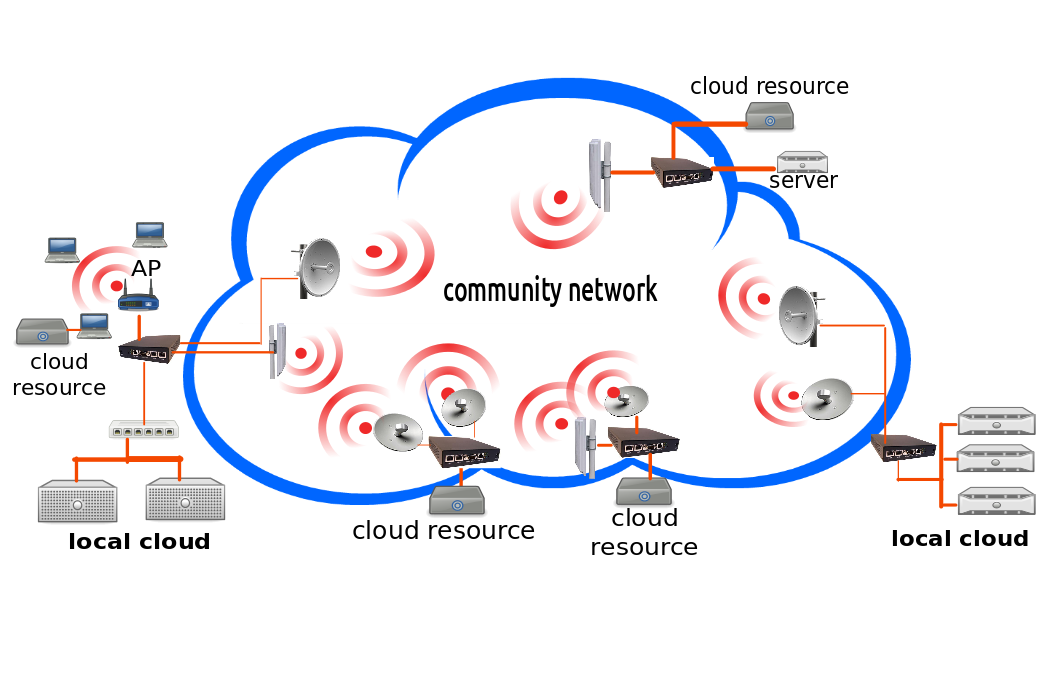
\includegraphics[width=0.65\textwidth,keepaspectratio]{com_node}
%	\caption{Nodes in a community network}
%	\label{fig:community-network}
%\end{figure}

%%%%%%%%%%%%%%%%%%%%%%%%%%%%%%%%%%%%%%%%%%%%
\subsection{Community Cloud Scenarios}

These observed characteristics of the community networks lead to two cloud scenarios in our model, 
local and federated community clouds.
The SNs and ONs provide the networking infrastructure, which in order to realise the community cloud, need to be attached to other hardware like servers and storage.
The cloud management software will run on these servers attached to the networking nodes, SNs and ONs.
In the following, when we refer to these nodes, SNs or ONs, we presume them to be 
those networking nodes of the community networks 
that already have other computing hardware attached.

First, we have the \enquote{local community cloud} scenario, 
which is derived from the topology of the community network, given by the fact that 
the community network generally has two different types of nodes, SNs and ONs, 
and the observed characteristics of the strength of social network within zones~\cite{Vega2012}. 
In such a local community cloud, a SN is responsible for the management of a set of attached nodes contributing cloud resources. 
From the perspective of the attached nodes, this SN acts as a centralised unit to manage the cloud services. 

Next, we consider the scenario when multiple SNs from different zones in a community network connect to form a \enquote{federated community cloud}.
SNs connect physically with other SNs through wireless links and logically in an overlay network to other SNs that manage local clouds.
SNs coordinate among themselves for provisioning infrastructure service so the requests originating from one SN's zone can be satisfied by the resources allocated from another SN's zone.
Figure~\ref{fig:federated_cloud} shows an example of a federated community cloud formed by SNs from three zones.
The ONs in a given zone are directly managed by the SN in that zone but they can also consume resources from other zones because of the coordination among SNs.

%% FIGURE
\begin{figure}[tbp]
	\centering
	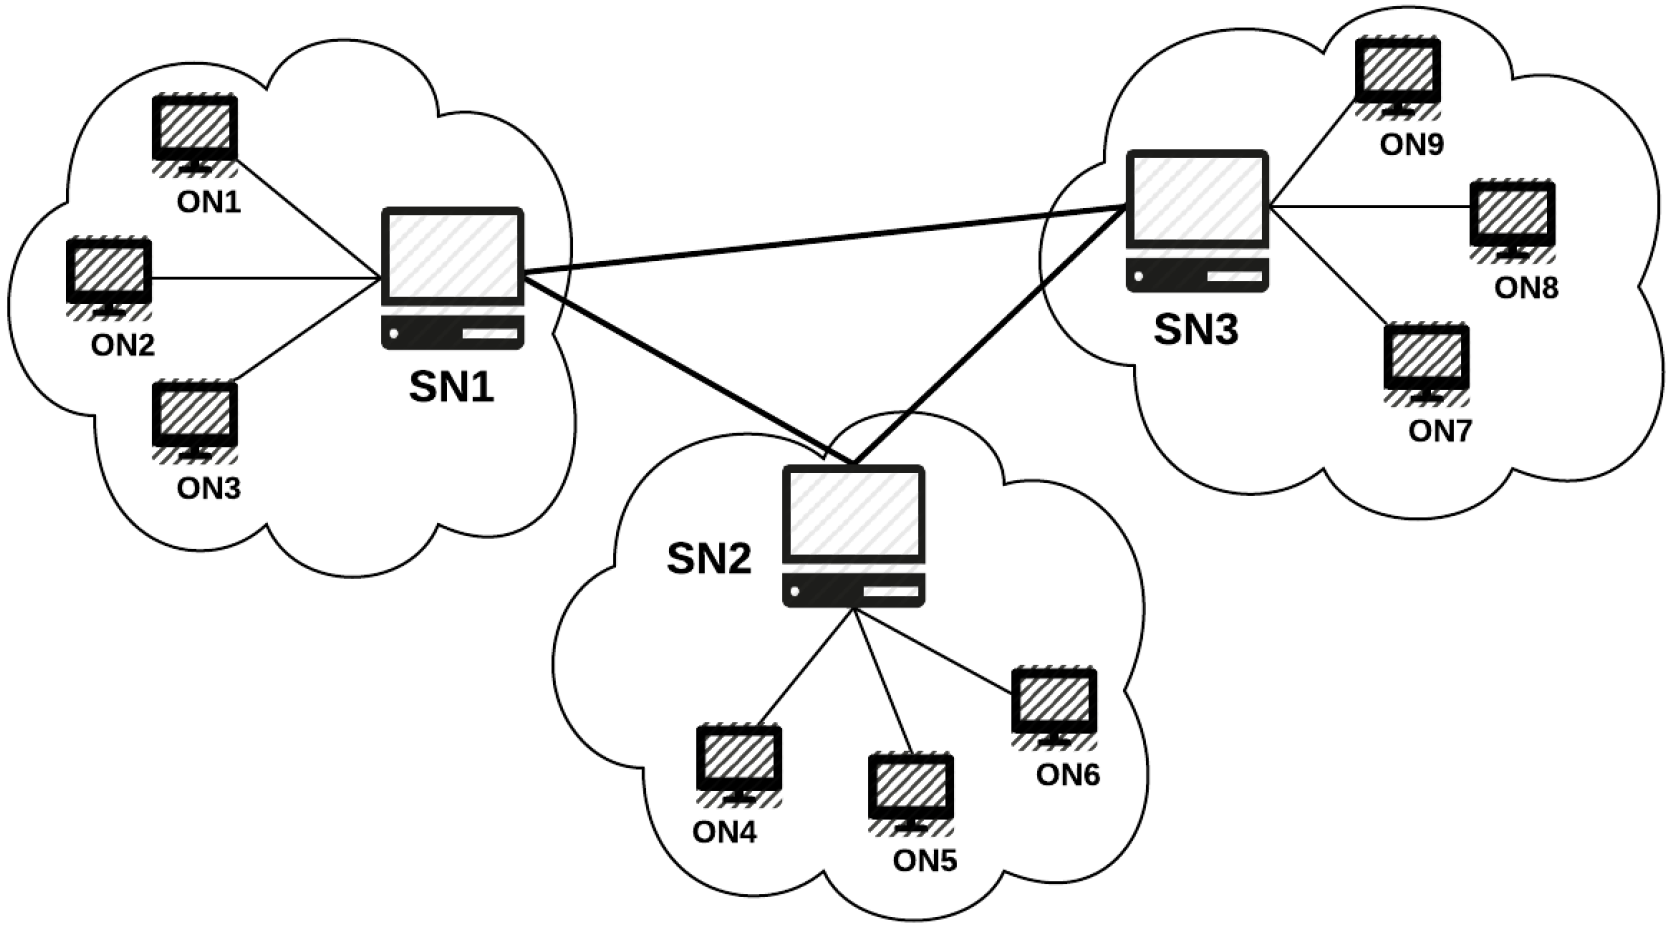
\includegraphics[width=0.75\textwidth,keepaspectratio]{federated_cloud}
	\caption{Nodes in federated community cloud}
	\label{fig:federated_cloud}
\end{figure}

%%%%%%%%%%%%%%%%%%%%%%%%%%%%%%%%%%%%%%%%%%%%
%\subsection{Resource Provisioning Model}
\subsection{Resource Provisioning and Coordination}

With these two cloud scenarios, we assume that requests for the resources are generated by the users at the ONs.
Users, who want to contribute resources also make them available at ONs.
All the requests are submitted directly to the single SN managing that particular ON.
SN keeps track of all the ONs, the available resources, and the requests from the users.
SN services the requests depending on the availability of the resources, 
and whether the user has sufficient credit to pay for these resources. 
When a user consumes resources at another ON, the connection is set up through the SN, and all the interactions remain within the local community cloud.
When SN decides to federate resources with other zones of community clouds, all the interactions are through the SNs of both the zones.



